\documentclass[12pt]{article}

% CSCE 763 template style adapted for EMCH homework
\usepackage{amsmath}
\usepackage{amssymb}
\usepackage{amsfonts}
\usepackage{graphicx}
\usepackage{tikz}
\usepackage{pgfplots}
\usepackage[margin=1in]{geometry}
\usepackage{xcolor}
\usepackage{enumitem}
\usepackage{tcolorbox}
\usepackage{fancyhdr}
\usepackage{booktabs}
\usepackage{array}
\usepackage{colortbl}
\usepackage{float}
\usepackage{tabularx}
\usepackage{multicol}
\usepackage{listings}

\pgfplotsset{compat=1.17}
\usetikzlibrary{shapes.geometric, arrows.meta, positioning, patterns}

% --- USC Brand Colors (from CSCE 763 template) ---
\definecolor{USC_Garnet}{HTML}{73000A}
\definecolor{USC_Sandstorm}{HTML}{FFF2E3}
\definecolor{USC_Black90}{HTML}{363636}
\definecolor{USC_Black70}{HTML}{5C5C5C}
\definecolor{USC_Black50}{HTML}{A2A2A2}
\definecolor{USC_Black10}{HTML}{ECECEC}
\definecolor{USC_Honeycomb}{HTML}{65780B}
\definecolor{USC_Atlantic}{HTML}{466A9F}
\definecolor{USC_Congaree}{HTML}{1F414D}
\definecolor{USC_Rose}{HTML}{CC2E40}

\pagestyle{fancy}
\setlength{\headheight}{14.5pt}
\fancyhf{}
\fancyhead[L]{Page \thepage}
\fancyhead[C]{CSCE 763}
\fancyhead[R]{JC Vaught}
\renewcommand{\headrulewidth}{0pt}

\newtcolorbox{stepbox}[1][Step]{
  colback=white,
  colframe=USC_Garnet,
  fonttitle=\bfseries,
  title=#1,
  sharp corners,
  colbacktitle=USC_Garnet,
  coltitle=white,
}

\newtcolorbox{resultsbox}{
  colback=white,
  colframe=USC_Honeycomb,
  fonttitle=\bfseries,
  title=Results,
  sharp corners,
  colbacktitle=USC_Honeycomb,
  coltitle=white,
}

\newcommand{\question}[1]{%
  \clearpage
  \vspace{0.5cm}
  {\noindent\normalsize \textbf{#1}}
  \vspace{0.2cm}
  \hrule
  \vspace{0.1cm}
  \hrule
  \vspace{0.3cm}
}

\newcommand{\questionpart}[1]{%
  \clearpage
  \vspace{0.5cm}
  {\noindent\normalsize \textbf{#1}}
  \vspace{0.2cm}
  \hrule
  \vspace{0.1cm}
  \hrule
  \vspace{0.3cm}
}

\setlist[enumerate,1]{label=\arabic*.}
\setlist[enumerate,2]{label=(\alph*)}

\lstset{language=Matlab,
        basicstyle=\ttfamily\small,
        keywordstyle=\color{blue},
        commentstyle=\color{gray},
        stringstyle=\color{red},
        breaklines=true,
        frame=single,
        showstringspaces=false,
        numbers=left,
        numberstyle=\tiny\color{gray},
        stepnumber=1}

\graphicspath{{./}{figures/}}
\title{EMCH 367 Controls \\ Homework \#2}
\author{Jacob C. Vaught}
\date{Fall 2024}

\begin{document}
\maketitle
\setlength{\parindent}{0pt}

\begin{center}
\begin{tcolorbox}[colback=white, colframe=gray!50!black, colbacktitle=gray!20!white,
                  coltitle=black, sharp corners, boxrule=1pt,
                  title=\Large\bfseries Table of Contents]
\begin{tabular}{p{0.82\textwidth}r}
\textbf{Problem 1 (20pt)} \dotfill & \textbf{\pageref{quest:1}} \\[0.3em]
\textbf{Problem 2 (20pt)} \dotfill & \textbf{\pageref{quest:2}} \\[0.3em]
\textbf{Problem 3 (40pt)} \dotfill & \textbf{\pageref{quest:3}} \\[0.3em]
\textbf{Problem 4 (20pt)} \dotfill & \textbf{\pageref{quest:4}} \\[0.3em]
\textbf{Bonus Problem (20pt)} \dotfill & \textbf{\pageref{quest:5}} \\n\end{tabular}
\vspace{0.2cm}
\end{tcolorbox}
\end{center}


\question{Problem 1 (20pt)}\label{quest:1}
\begin{stepbox}[Step 1: Approach]
Work through each requested subpart and show supporting derivations.
\end{stepbox}

\textbf{True or False}
\begin{enumerate}
	\item Damper element stores the energy. \newline
	      \textcolor{blue}{False: A damper dissipates energy, typically through heat, rather than storing it.}
	\item Underdamped system has damping ratio between 0 and 1. \newline
	      \textcolor{blue}{True: An underdamped system oscillates with a damping ratio \( 0 < \zeta < 1 \).}
	\item The stability of a 2nd order system depends on the sign of real part of the poles of the transfer function. \newline
	      \textcolor{blue}{True: Stability is determined by whether the real part of the poles is negative (stable) or positive (unstable).}
	\item If the step response is stable, then the ramp response is stable. \newline
	      \textcolor{blue}{False: Stability for a step response does not guarantee stability for a ramp input, as they involve different responses.}
	\item Steady state error is a specific performance indicator. \newline
	      \textcolor{blue}{True: Steady-state error measures the difference between the system output and the desired input in the long term.}
	\item For a second order system, overshoot always occurs. \newline
	      \textcolor{blue}{False: Overshoot only occurs in underdamped systems; critically damped or overdamped systems do not overshoot.}
	\item Settling time is always greater than or equal to rise time. \newline
	      \textcolor{blue}{False: Settling time typically includes time for the system to oscillate and dampen, making it longer than the rise time SOMETIMES.}
	\item Laplace transformation exists for all time functions. \newline
	      \textcolor{blue}{False: The Laplace transform exists only for functions that meet certain conditions, such as being piecewise continuous and of exponential order.}
	\item Initial value theorem can be used to find steady-state error. \newline
	      \textcolor{blue}{False: The initial value theorem is used to find the initial value of a function, not the steady-state error.}
	\item Impulse response is the system response with respect to the impulse input. \newline
	      \textcolor{blue}{True: The impulse response represents how a system reacts to a delta function input (impulse).}
\end{enumerate}

\begin{center}
	\noindent % Ensures the table spans the text width starting from the left margin
	\begin{tabularx}{\textwidth}{|*{10}{X|}} % Creates 10 equal-width columns that fill the page
		\hline
		Q1 & Q2 & Q3 & Q4 & Q5 & Q6 & Q7 & Q8 & Q9 & Q10 \\ \hline
		F  & T  & T  & F  & T  & F  & F  & F  & F  & T   \\ 
		\hline
	\end{tabularx}
\end{center}

\newpage
\begin{resultsbox}
Final answers for the previous problem are summarized in the work above.
\end{resultsbox}

\question{Problem \#2 (20pt)}\label{quest:2}
\begin{stepbox}[Step 1: Approach]
Work through each requested subpart and show supporting derivations.
\end{stepbox}

\begin{figure}[h]
	\centering
	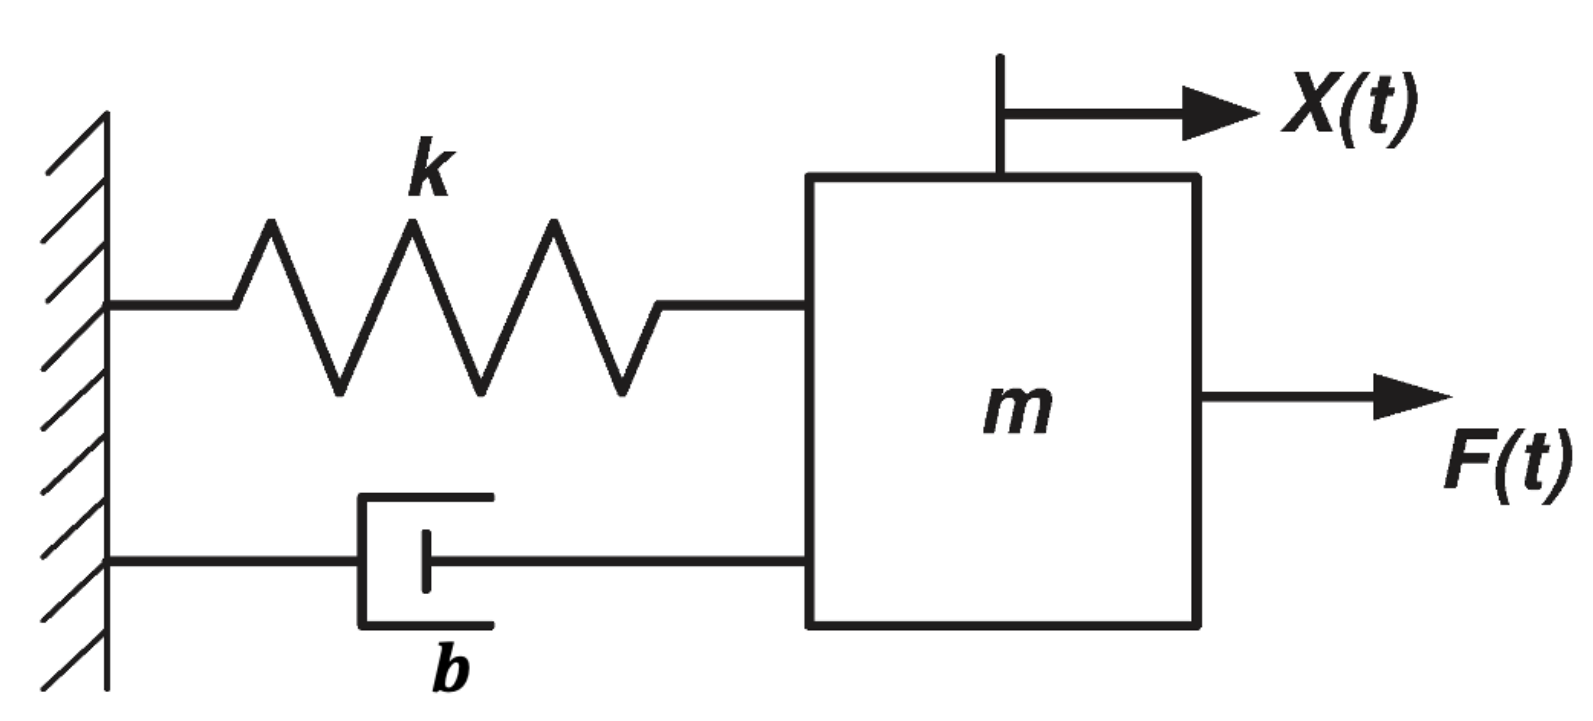
\includegraphics[width=0.6\textwidth]{p1.png}
	\caption{Spring-Mass-Damper System}
\end{figure}

Consider the spring-mass-damper system shown in Figure 1 with the following parameters:

\begin{itemize}
	\item Mass, $m = 1 \text{ kg}$
	\item Spring constant, $k = 100 \text{ N/m}$
	\item Damping coefficient, $b = 8 \text{ N}\cdot\text{s/m}$
\end{itemize}

\subsection*{(a) Transfer Function Derivation}
The equation of motion for the system is given by:

\begin{equation*}
	m\ddot{x}(t) + b\dot{x}(t) + kx(t) = F(t)
\end{equation*}

Taking the Laplace transform of the equation (assuming zero initial conditions):

\begin{equation*}
	m s^2 X(s) + b s X(s) + k X(s) = F(s)
\end{equation*}

Rearranging to solve for the transfer function $G(s) = \frac{X(s)}{F(s)}$:

\begin{equation*}
	\textcolor{blue}{G(s) = \frac{1}{m s^2 + b s + k}}
\end{equation*}

\newpage
\subsection*{(b) Step Response in MATLAB}
The MATLAB code to plot the step response for 5 seconds is as follows:

\begin{verbatim}
% Parameters
m = 1;
b = 8;
k = 100;

% Transfer Function
num = 1;
den = [m b k];
sys = tf(num, den);

% Step Response for 5 seconds
figure;
step(sys, 5);
title('Step Response of the System');
xlabel('Time (s)');
ylabel('Amplitude');
grid on;
saveas(gcf, 's1.png');
\end{verbatim}

\begin{figure}[h]
	\centering
	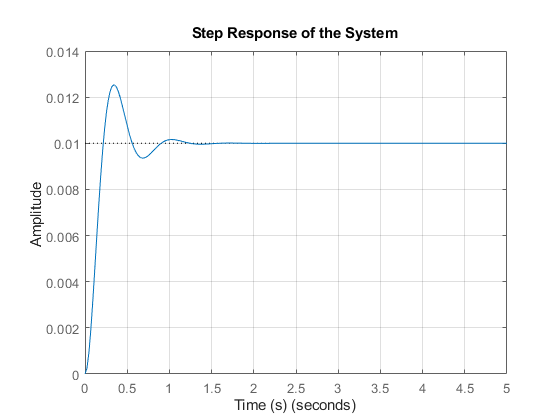
\includegraphics[width=0.6\textwidth]{s1.png}
	\caption{Step Response of the System}
\end{figure}
\newpage
\subsection*{(c) Cosine Input Response in MATLAB}
The MATLAB code to plot the response to the cosine input $f(t) = \cos(\omega t)$ with $\omega = \frac{\pi}{2}$ s$^{-1}$ for 10 seconds is as follows:

\begin{verbatim}
% Parameters
omega = pi / 2;
t = 0:0.01:10; % Time vector from 0 to 10 seconds

% Cosine Input
f_t = cos(omega * t);

% Response to Cosine Input
[y, t_out] = lsim(sys, f_t, t);

% Plotting
figure;
plot(t, f_t, 'r--', 'DisplayName', 'Input: cos(omega t)');
hold on;
plot(t_out, y, 'b', 'DisplayName', 'System Response');
title('System Response to cos(omega t) Input');
xlabel('Time (s)');
ylabel('Amplitude');
legend show;
grid on;
saveas(gcf, 's2.png');
\end{verbatim}

\begin{figure}[h!]
	\centering
	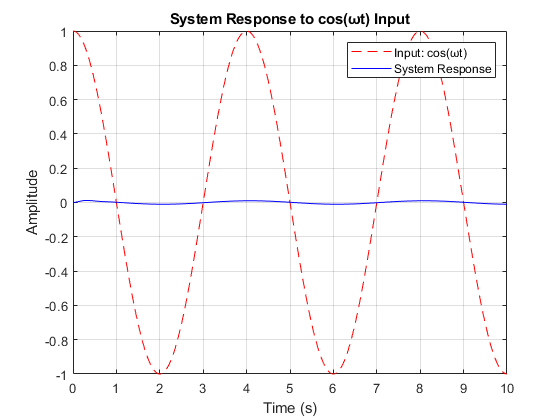
\includegraphics[width=0.6\textwidth]{s2.png}
	\caption{System Response to Cosine Input}
\end{figure}

\newpage
\subsection*{(d) Cosine Input Response in SimuLink}

\begin{figure}[h]
	\centering
	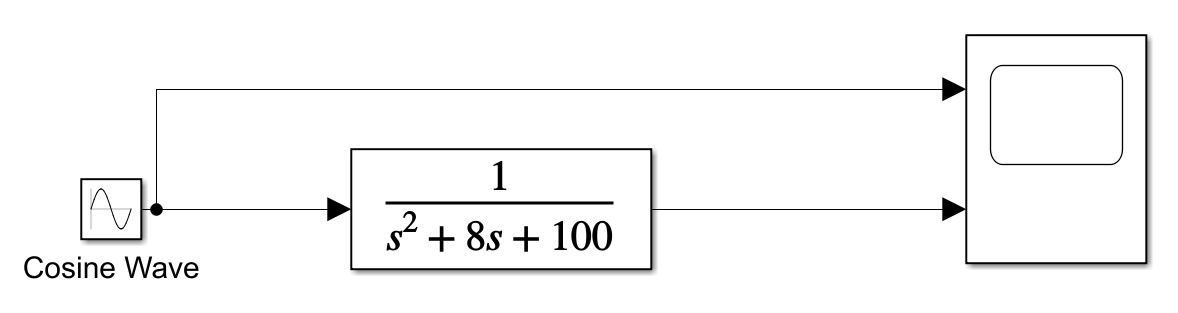
\includegraphics[width=0.6\textwidth]{s3a.png}
	\caption{Block System}
\end{figure}
\begin{figure}[h]
	\centering
	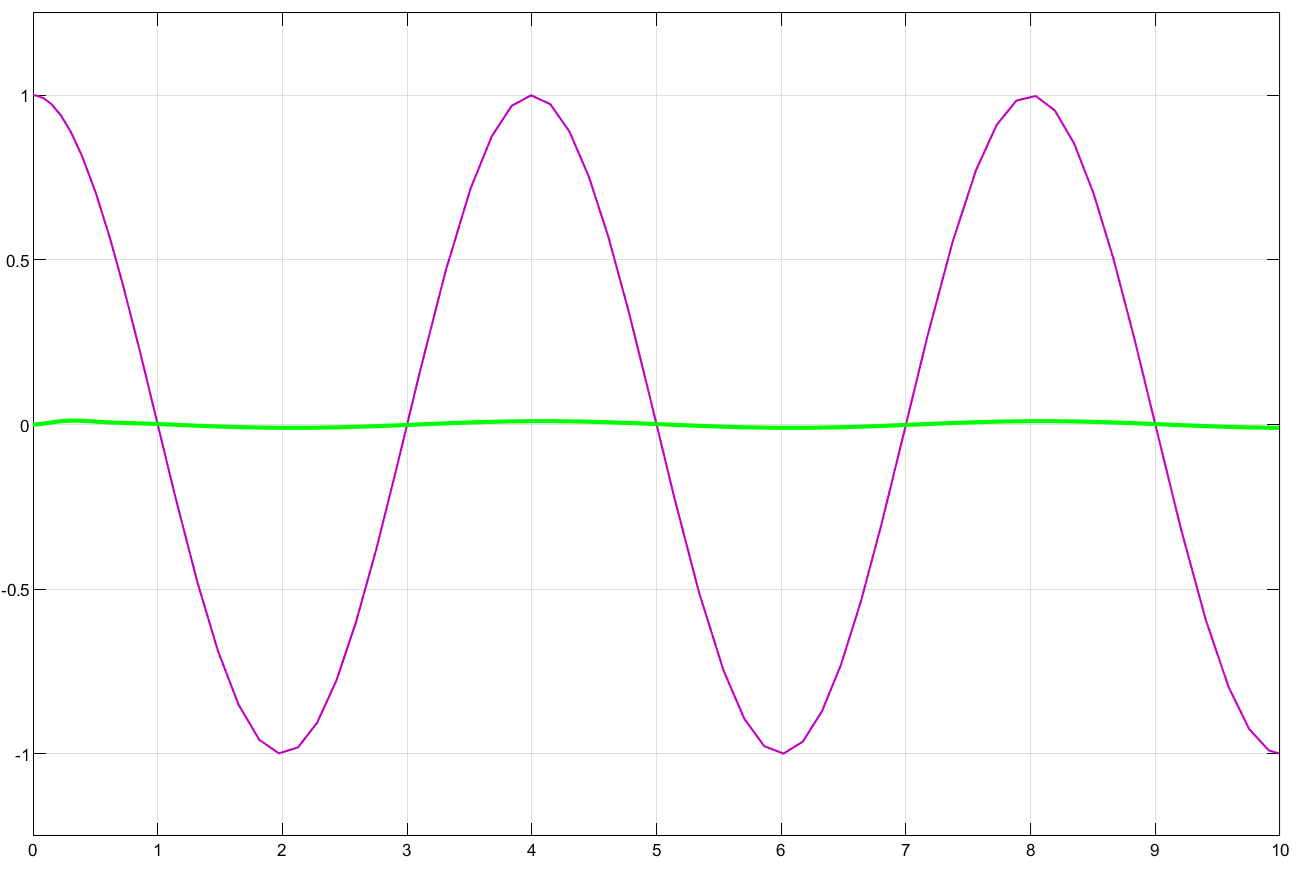
\includegraphics[width=0.6\textwidth]{s3b.png}
	\caption{System Response to Cosine Input}
\end{figure}

\newpage
\begin{resultsbox}
Final answers for the previous problem are summarized in the work above.
\end{resultsbox}

\question{Problem 3. (40 pt) Higher Order System}\label{quest:3}
\begin{stepbox}[Step 1: Approach]
Work through each requested subpart and show supporting derivations.
\end{stepbox}


\subsection*{(a) (20 pt)] Consider the system and find the TF of the system $\frac{Y(s)}{U(s)}$ with zero initial conditions.}


\begin{figure}[h]
	\centering
	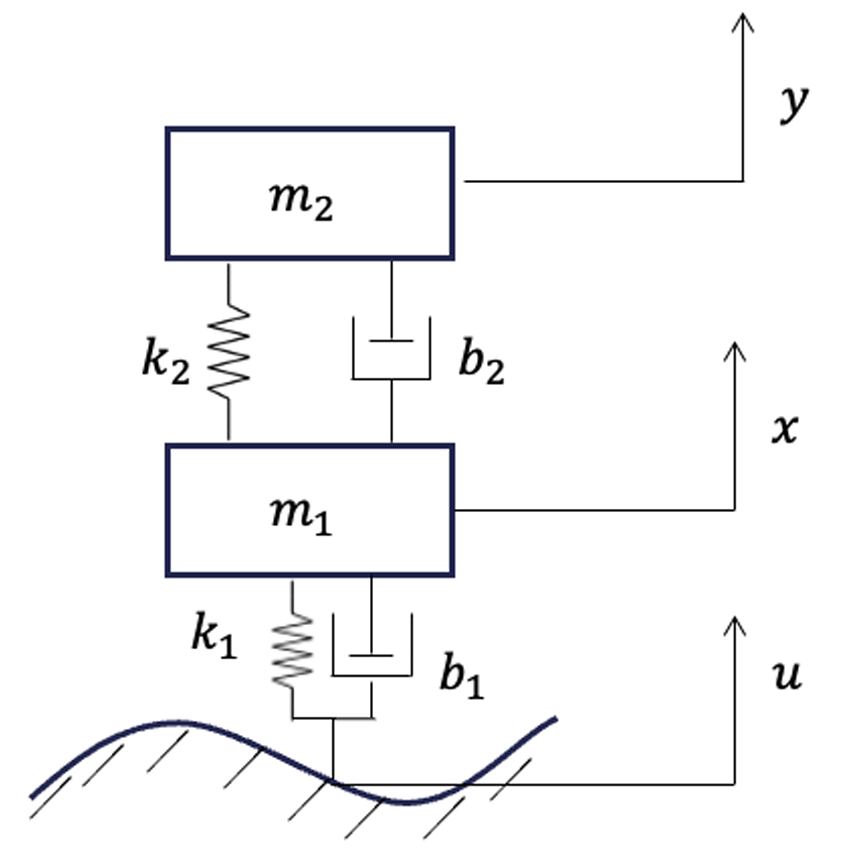
\includegraphics[width=0.4\textwidth]{p3.png} % Replace with the correct path to your image
	\caption{Suspension System}
	\label{fig:suspension_system}
\end{figure}

Solving for each mass independently, equations to model each mass can be derived(note that the signs for the mass in question remain the same).

\begin{equation*}
	\begin{aligned}
		m_1 \ddot{x} & = k_2 (y - x) + b_2 (\dot{y} - \dot{x}) + k_1 (u - x) + b_1 (\dot{u} - \dot{x}) \quad \text{(Eq. 1)} \\
		m_2 \ddot{y} & = k_2 (x - y) + b_2 (\dot{x} - \dot{y}) \quad \text{(Eq. 2)}                                         
	\end{aligned}
\end{equation*}

Hence, we can derive the following equations:

\begin{equation*}
	\begin{aligned}
		m_1 \ddot{x} + (b_1 + b_2) \dot{x} + (k_1 + k_2) x & = b_2 \dot{y} + b_1 \dot{u} + k_1 u \quad \text{(Eq. 3)} \\
		m_2 \ddot{y} + b_2 \dot{y} + k_2 y                 & = b_2 \dot{x} + k_2 x \quad \text{(Eq. 4)}               
	\end{aligned}
\end{equation*}

Taking the Laplace transform:

\begin{equation*}
	\begin{aligned}
		(m_1 s^2 + (b_1 + b_2)s + (k_1 + k_2))X(s) & = b_2 s Y(s) + (b_1 s + k_1) U(s) \quad \text{(Eq. 5)} \\
		(m_2 s^2 + b_2 s + k_2)Y(s)                & = (b_2 s + k_2) X(s) \quad \text{(Eq. 6)}              
	\end{aligned}
\end{equation*}

Using Eq. (6) to solve for \( X(s) \), we get:

\begin{equation*}
	\textcolor{blue}{X(s) = \frac{m_2 s^2 + b_2 s + k_2}{b_2 s + k_2}Y(s)} \quad \text{(Eq. 7)}
\end{equation*}

Combining into Eq. (5) to eliminate \( X(s) \), we get:

\begin{equation*}
	\left[ m_1 s^2 + (b_1 + b_2) s + (k_1 + k_2) \right] \left( \frac{m_2 s^2 + b_2 s + k_2}{b_2 s + k_2} \right) Y(s)  = (b_2 s + k_2) Y(s) + (b_1 s + k_1) U(s) \quad \text{(Eq. 8)}
\end{equation*}

Simplifying further:

\begin{equation*}
	\left[ \frac{[m_1 s^2 + (b_1 + b_2) s + (k_1 + k_2)]\cdot [m_2 s^2 + b_2 s + k_2]}{(b_2 s + k_2)} \right] Y(s) = (b_2 s + k_2) Y(s) + (b_1 s + k_1) U(s) \quad \text{(Eq. 9)}
\end{equation*}

Getting \( Y(s) \) on one side:

\begin{equation*}
	\left[ \frac{[m_1 s^2 + (b_1 + b_2) s + (k_1 + k_2)]\cdot [m_2 s^2 + b_2 s + k_2]}{(b_2 s + k_2)} - (b_2 s + k_2) \right] Y(s) = (b_1 s + k_1) U(s)
\end{equation*}

Finally, solving for \( \frac{Y(s)}{U(s)} \):

\begin{equation*}
	\textcolor{blue}{\frac{Y(s)}{U(s)} = \frac{(b_1 s + k_1) (b_2 s + k_2)}{(m_1 s^2 + (b_1 + b_2) s + (k_1 + k_2))(m_2 s^2 + b_2 s + k_2) - (b_2 s + k_2)^2}} \quad \text{(Eq. 10)}
\end{equation*}

\subsection*{(b) (10 pt) Is the system stable?}
Due to the system approaching 0 and 1 respectively, the system is stable.
\subsection*{(c) System Stability Analysis + (d) Impulse and Step Responses for 100 Seconds}

\begin{figure}[h!]
	\centering
	\begin{minipage}[t]{0.48\textwidth}
		\centering
		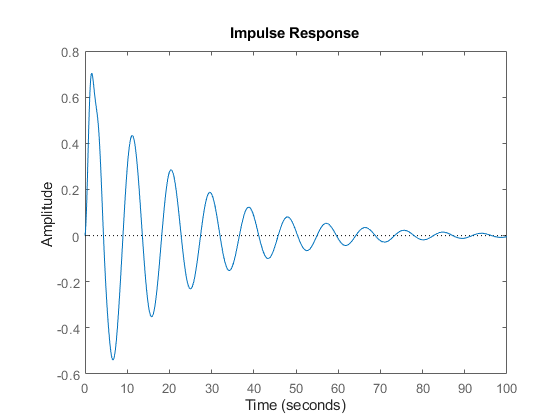
\includegraphics[width=0.8\textwidth]{s3ir.png}
		\caption{Impulse Response over 100 Seconds}
	\end{minipage}
	\hfill
	\begin{minipage}[t]{0.48\textwidth}
		\centering
		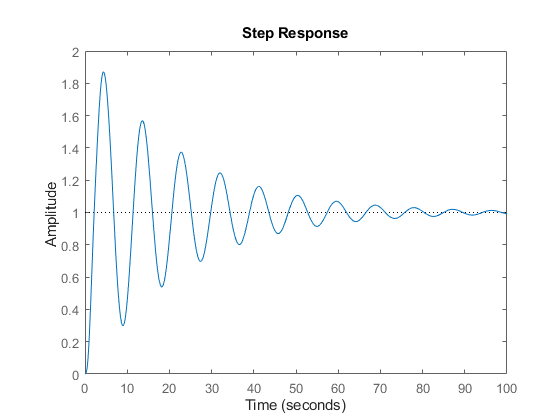
\includegraphics[width=0.8\textwidth]{s3sr.png}
		\caption{Step Response over 100 Seconds}
	\end{minipage}
\end{figure}

% Column 1
\textbf{MATLAB Code for Stability Analysis:}
\begin{verbatim}
    % System parameters
    m1 = 100;
    m2 = 100;
    k1 = 100;
    k2 = 400;
    b1 = 20;
    b2 = 50;

    % Define the transfer function using symbolic variable s
    s = tf('s');
    Y_over_U = (b1 * s + k1) * (b2 * s + k2) / ...
              ((m1 * s^2 + (b1 + b2) * s + (k1 + k2)) * (m2 * s^2 + b2 * s + k2) - (b2 * s + k2)^2);

    % Time vector for 100 seconds
    t = 0:0.1:100;
    
    % Impulse Response
    figure;
    impulse(Y_over_U, t);
    title('Impulse Response over 100 Seconds');
    xlabel('Time (seconds)');
    ylabel('Amplitude');
    grid on;
    saveas(gcf, 'impulse_response.png');
    
    % Step Response
    figure;
    step(Y_over_U, t);
    title('Step Response over 100 Seconds');
    xlabel('Time (seconds)');
    ylabel('Amplitude');
    grid on;
    saveas(gcf, 'step_response.png');
\end{verbatim}


\newpage
\newpage
\begin{resultsbox}
Final answers for the previous problem are summarized in the work above.
\end{resultsbox}

\question{Problem \#4 (20pt) Performance indicators of 2nd order system.}\label{quest:4}
\begin{stepbox}[Step 1: Approach]
Work through each requested subpart and show supporting derivations.
\end{stepbox}

\subsection*{(a) For step response, find rise time, settling time, overshoot, peak time, and peak value.}
Consider a spring-mass-damper system characterized by the differential equation:

\[
	\ddot{x} + 8\dot{x} + 36x = 36f(t)
\]
\[
	s^2 X(s) + 8s X(s) + 36X(s) = 36F(s)
\]

For a step input \( f(t) = u(t) \), the Laplace transform is:

\[
	F(s) = \frac{1}{s}
\]

\[
	\frac{X(s)}{F(s)} = \frac{36}{s(s^2 + 8s + 36)}
\]

This can be expressed in the standard second-order form:

\[
	\frac{X(s)}{F(s)} = \frac{\omega_n^2}{s(s^2 + 2\zeta\omega_n s + \omega_n^2)}
\]

Comparing coefficients, the natural frequency and damping ratio are found to be:

\[
	\textcolor{blue}{\omega_n = \sqrt{36} = 6 \, \text{rad/s}}
\]

\[
	2\zeta\omega_n = 8 \quad \Rightarrow \quad \textcolor{blue}{\zeta = \frac{8}{2 \times 6} = \frac{2}{3}}
\]

The \textbf{peak time} \( t_p \) is given by:

\[
	\textcolor{blue}{t_p = \frac{\pi}{\omega_n \sqrt{1 - \zeta^2}} = \frac{\pi}{6 \sqrt{1 - \left(\frac{2}{3}\right)^2}} = \frac{\pi}{4.4724} \approx 0.702 \, \text{seconds}}
\]

The \textbf{percentage overshoot} \( M_p \) is:

\[
	\textcolor{blue}{M_p = e^{-\frac{\zeta \pi}{\sqrt{1 - \zeta^2}}} \times 100\% = e^{-\frac{\frac{2}{3} \times \pi}{\sqrt{\frac{5}{9}}}} \approx 6.04\%}
\]

The \textbf{settling time} \( t_s \) (for 2\% tolerance) is:

\[
	\textcolor{blue}{t_s = \frac{4}{\zeta \omega_n} = \frac{4}{\frac{2}{3} \times 6} = 1 \, \text{second}}
\]

The \textbf{rise time} \( t_r \) can be approximated as:

\[
	\textcolor{blue}{t_r \approx \frac{\pi - \tan^{-1} \left( \frac{\sqrt{1 - \zeta^2}}{\zeta} \right)}{\omega_n \sqrt{1 - \zeta^2}} \approx \frac{2.3038}{4.4724} \approx 0.515 \, \text{seconds}}
\]

The \textbf{peak value} \( x_p \) is given by:

\[
	\textcolor{blue}{x_p = 1 + M_p \approx 1 + 0.0604 = 1.0604}
\]

The performance indicators are summarized in Table~\ref{tab:performance_indicators}.
\begin{table}[h!]
	\centering
	\begin{tabular}{@{}ll@{}}
		\toprule
		\textbf{Performance Indicator} & \textbf{Value}    \\ \midrule
		Rise Time (\( t_r \))          & $\approx 0.515$ s \\
		Peak Time (\( t_p \))          & $\approx 0.702$ s \\
		Overshoot (\( M_p \))          & $\approx 6.04\%$  \\
		Settling Time (\( t_s \))      & $\approx 1$ s     \\
		Peak Value (\( x_p \))         & $\approx 1.0604$  \\ \bottomrule
	\end{tabular}
	\caption{Performance Indicators of the Second-Order System}
	\label{tab:performance_indicators}
\end{table}

\newpage
\subsection*{(b) Find the steady state error of the ramp response.}
To determine the steady-state error (\( e_{ss} \)) for a ramp input using the final value theorem, we start with the given system:

\[
	\frac{X(s)}{F(s)} = \frac{36}{s^2 + 8s + 36}
\]

For a ramp input, \( f(t) = t \), the Laplace transform is:

\[
	F(s) = \frac{1}{s^2}
\]

We find \( X(s) \) by multiplying the transfer function by \( F(s) \):

\[
	X(s) = \frac{X(s)}{F(s)} \cdot F(s) = \frac{36}{s^2 + 8s + 36} \cdot \frac{1}{s^2} = \frac{36}{s^2 (s^2 + 8s + 36)}
\]

The steady-state error is defined as:

\[
	e_{ss} = \lim_{t \to \infty} (f(t) - x(t)) = \lim_{s \to 0} s \left[ F(s) - X(s) \right]
\]

Substitute \( F(s) \) and \( X(s) \):

\[
	e_{ss} = \lim_{s \to 0} s \left[ \frac{1}{s^2} - \frac{36}{s^2 (s^2 + 8s + 36)} \right]
\]

Simplify the expression:

\[
	e_{ss} = \lim_{s \to 0} \left[ \frac{1}{s} - \frac{36}{s (s^2 + 8s + 36)} \right]
\]

\[
	e_{ss} = \lim_{s \to 0} \frac{s^2 + 8s + 36 - 36}{s (s^2 + 8s + 36)}
\]

\[
	e_{ss} = \lim_{s \to 0} \frac{s^2 + 8s}{s (s^2 + 8s + 36)} = \lim_{s \to 0} \frac{s + 8}{s^2 + 8s + 36}
\]

Evaluating the limit:

\[
	\textcolor{blue}{e_{ss} = \frac{0 + 8}{0 + 0 + 36} = \frac{8}{36} = \frac{2}{9}}
\]

Thus, the steady-state error for a ramp input is:

\[
	\textcolor{blue}{e_{ss} = \frac{2}{9}}
\]

\newpage

\begin{resultsbox}
Final answers for the previous problem are summarized in the work above.
\end{resultsbox}

\question{Bonus Problem (20pt)}\label{quest:5}
\begin{stepbox}[Step 1: Approach]
Work through each requested subpart and show supporting derivations.
\end{stepbox}

In Problem 4, find the steady state error of the time response where f(t) = sin6t. (hint: The steady state error would not converge.)
\newline\newline
The steady-state error is defined as:
\begin{equation}
	e(t) = f(t) - x(t),
\end{equation}
where \( x(t) \) is the output of the system. Using the Final Value Theorem, the steady-state error is:
\begin{equation}
	e_{ss} = \lim_{t \to \infty} e(t) = \lim_{s \to 0} s E(s),
\end{equation}
where \( E(s) = F(s) - X(s) \).

The Laplace transform of the input signal \( f(t) = \sin(6t) \) is:
\begin{equation}
	F(s) = \frac{6}{s^2 + 36}.
\end{equation}

The output \( X(s) \) is given by:
\begin{equation}
	X(s) = \frac{36}{s^2 + 8s + 36} \cdot \frac{6}{s^2 + 36} = \frac{216}{(s^2 + 8s + 36)(s^2 + 36)}.
\end{equation}

The error signal in the Laplace domain is:
\begin{equation}
	E(s) = F(s) - X(s) = \frac{6}{s^2 + 36} - \frac{216}{(s^2 + 8s + 36)(s^2 + 36)}.
\end{equation}

For the steady-state error to converge, the limit \( \lim_{s \to 0} s E(s) \) must exist. However, due to the periodic nature of the sinusoidal input, the response \( x(t) \) will also oscillate indefinitely, causing \( e(t) \) to remain oscillatory. \textcolor{blue}{Thus, the steady-state error does not converge.}

\subsection*{MATLAB Verification}
To verify this behavior, we simulate the time-domain response using MATLAB. The following code generates the time response of the system and visualizes the error:

\begin{verbatim}
numerator = 36;
denominator = [1, 8, 36];
sys = tf(numerator, denominator);
t = 0:0.01:10; % Time vector from 0 to 10 seconds
input_signal = sin(6*t)'; % Input: sin(6t) transposed
output_signal = lsim(sys, input_signal, t);

figure;
subplot(2, 1, 1);
plot(t, input_signal, 'b', 'LineWidth', 1.5);
title('Input Signal: sin(6t)');
xlabel('Time (s)');
ylabel('Amplitude');

grid on;
subplot(2, 1, 2);
plot(t, output_signal, 'r', 'LineWidth', 1.5);
title('System Response');
xlabel('Time (s)');
ylabel('Amplitude');
grid on;

error_signal = input_signal - output_signal;
figure;
plot(t, error_signal, 'k', 'LineWidth', 1.5);
title('Error Signal: f(t) - x(t)');
xlabel('Time (s)');
ylabel('Amplitude');
grid on;
\end{verbatim}

The plots generated by the MATLAB script confirm that the error signal \( e(t) = f(t) - x(t) \) oscillates indefinitely and does not converge to a constant value.

\begin{figure}[h]
	\centering
	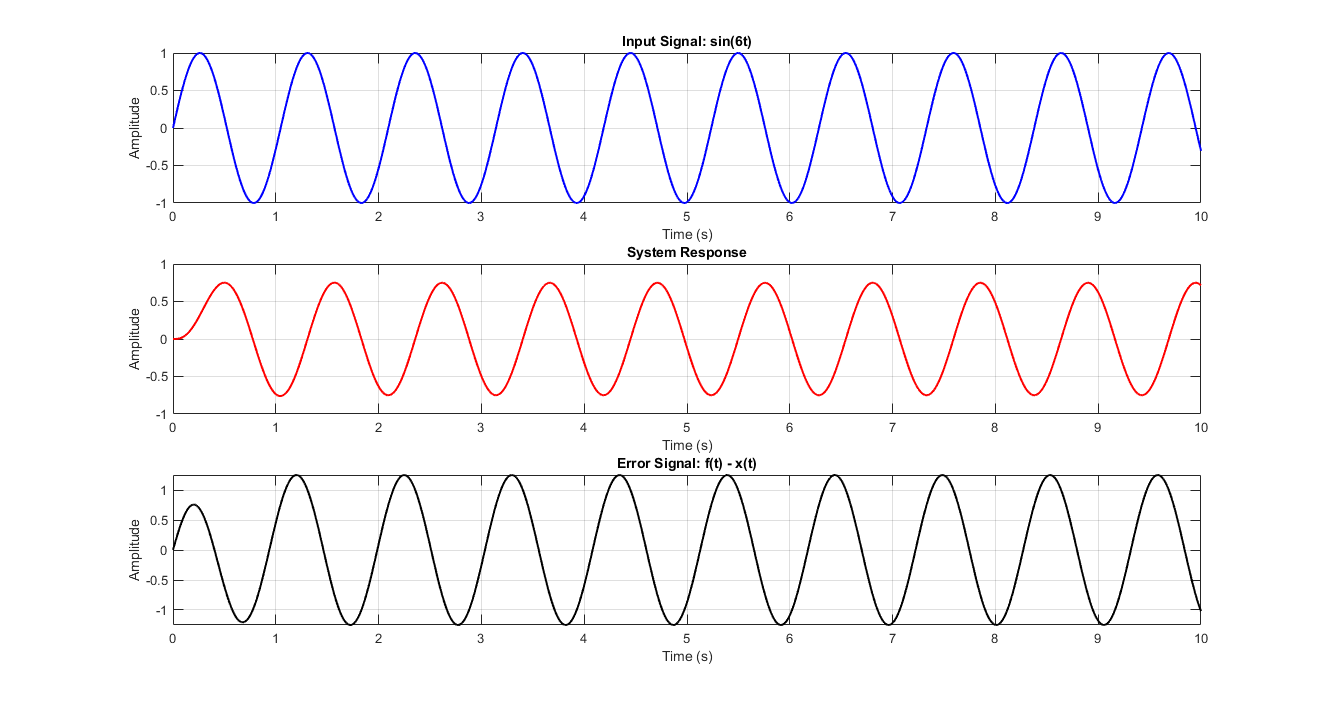
\includegraphics[width=0.95\textwidth]{sb.png}
	\caption{Time response of the system and the error signal for the input \( \sin(6t) \).}
	\label{fig:time_response}
\end{figure}

\begin{resultsbox}
Final answers for the previous problem are summarized in the work above.
\end{resultsbox}

\end{document}
